\documentclass[margin=5mm]{standalone}
\usepackage[utf8x]{inputenc}
\usepackage{amsmath}
\usepackage{tikz}
\usetikzlibrary{arrows, positioning}
\begin{document}
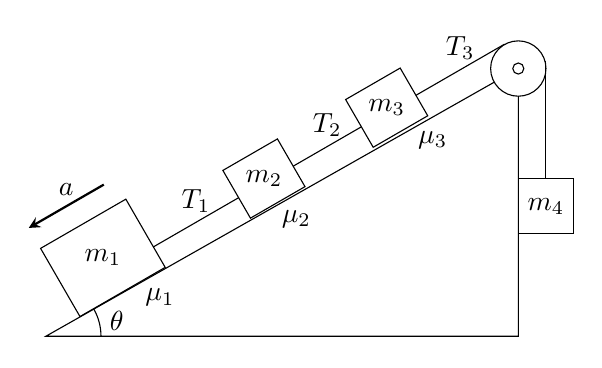
\begin{tikzpicture}
	\draw (0, 0) -- (6, 0) -- (6, 3.4) -- cycle;
    \draw (0.7, 0) arc (0:30:0.7);
    \node at (0.9, 0.2) {$\theta$};

    \begin{scope}[rotate=30]
    \draw (0.5, 0) rectangle (1.75, 1) node [pos=0.5] {$m_{1}$};
    \draw (1.75, 0.3) -- (3, 0.3) node [above, midway] {$T_{1}$};
    \draw (3, 0) rectangle (3.8, 0.7) node [pos=0.5] {$m_{2}$};
    \draw (3.8, 0.3) -- (4.8, 0.3) node [above, midway] {$T_{2}$};
    \draw (4.8, 0) rectangle (5.6, 0.7) node [pos=0.5] {$m_{3}$};
    \draw (5.6, 0.3) -- (6.9, 0.3) node [above, midway] {$T_{3}$};
    \draw [-stealth, thick] (1.6, 1.3) -- (0.5, 1.3) node [above, midway] {$a$};
    \node at (1.5, -0.3) {$\mu_{1}$};
    \node at (3.5, -0.3) {$\mu_{2}$};
    \node at (5.5, -0.3) {$\mu_{3}$};
    \end{scope}

    \draw [fill=white] (6, 3.4) circle (10pt);
    \draw [fill=white] (6, 3.4) circle (2pt);

    \draw (6.35, 3.5) -- (6.35, 2);
    \draw (6, 1.3) rectangle (6.7, 2) node [pos=0.5] {$m_{4}$};
\end{tikzpicture}
\end{document}